\section{Presentation Evaluation}

With my presentation complete, I reached out to peers, family members and industry experts to gather feedback on both my EPQ Artifact and my delivery of my presentation. I again utilised my self-built survey tool (with some recently improved graphing capabilities) to send out my survey to a wide audience. I received 33 responses in total, with a good mix of opinions. Each respondent had the opportunity to watch my presentation video for as long as they wished before the video

Please find my evaluation of the results below:

\begin{figure}[H]
    \centering
    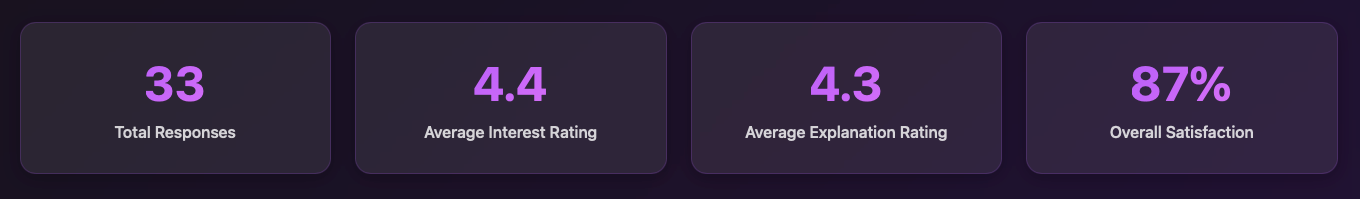
\includegraphics[width=0.8\textwidth]{VideoPresentation/PresentationEvaluation/media/overall.png}
    \caption{Result Summary}
\end{figure}

\subsection*{How interesting did you find the presentation?}

\begin{figure}[H]
    \centering
    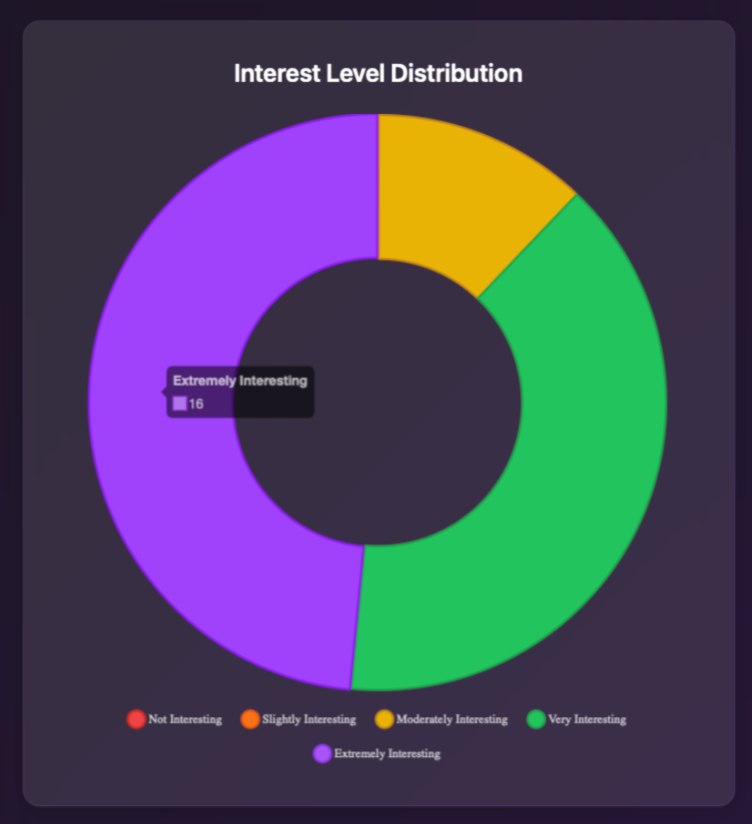
\includegraphics[width=0.6\textwidth]{VideoPresentation/PresentationEvaluation/media/interest.png}
    \caption{Visualisation of results}
\end{figure}

\subsection*{To what extent do you believe that I explained and evidenced my project?}

\begin{figure}[H]
    \centering
    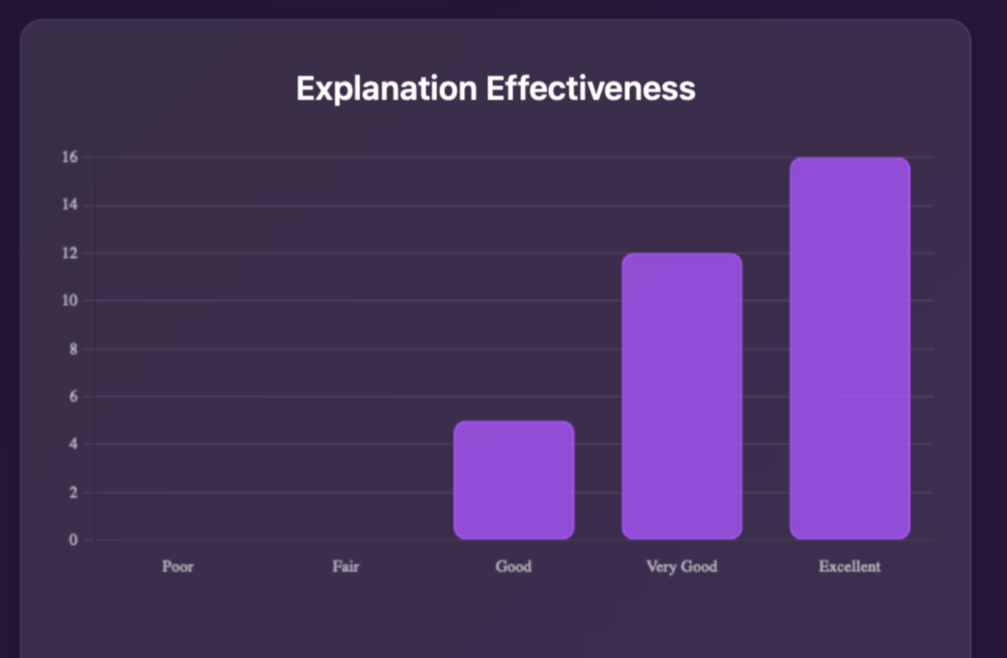
\includegraphics[width=0.6\textwidth]{VideoPresentation/PresentationEvaluation/media/explaination.png}
    \caption{Visualisation of results}
\end{figure}

\subsection*{How Well did I Demonstrate:}
\begin{itemize}
    \item Enthusiasm
    \item Confidence
    \item Knowledge and research
    \item Skill set development
    \item A visually appealing presentation
    \item Clear and concise delivery
\end{itemize}

\begin{figure}[H]
    \centering
    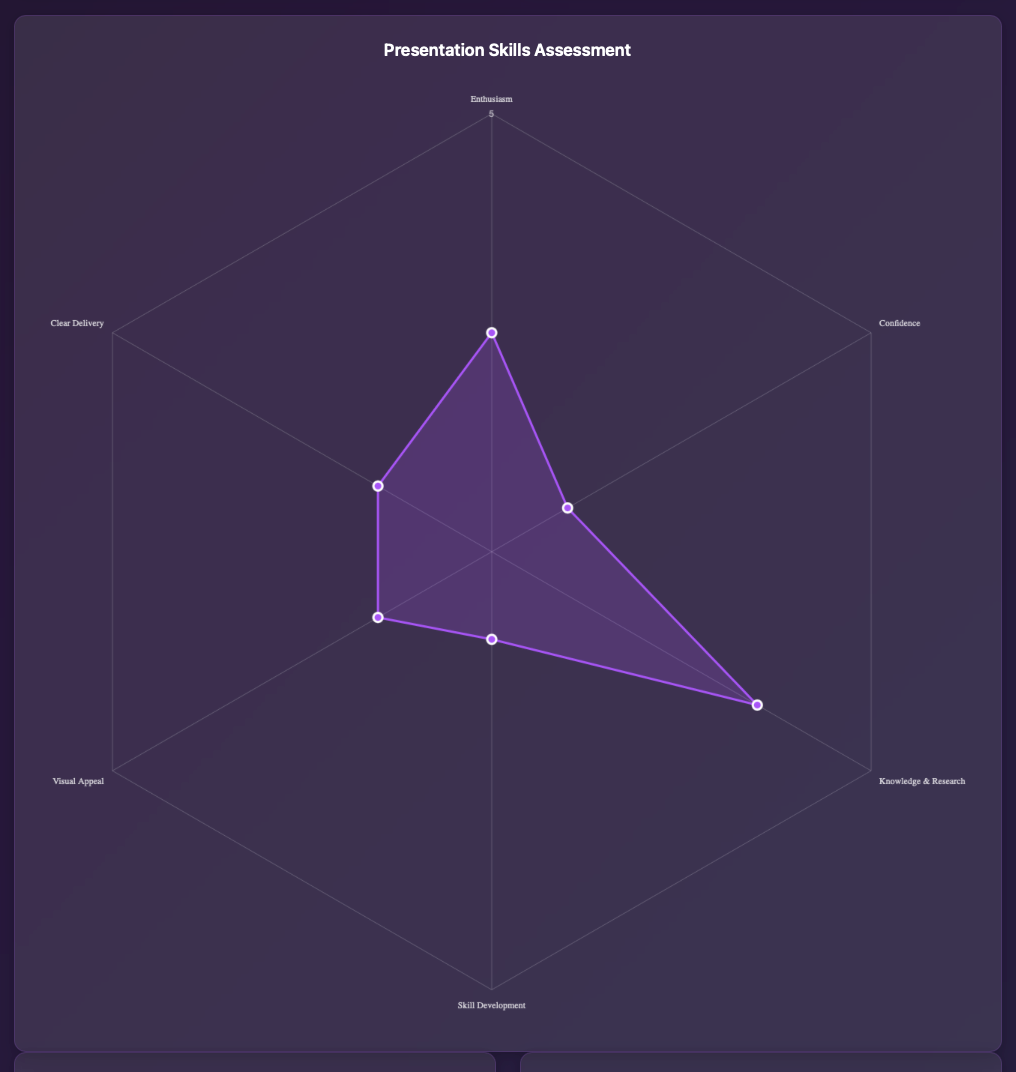
\includegraphics[width=0.6\textwidth]{VideoPresentation/PresentationEvaluation/media/skills.png}
    \caption{Visualisation of results}
\end{figure}

% \subsection*{Which was your favourite part of the presentation?}


% \subsection*{Are there any improvements you think I could make?}
\section*{Favourite Parts and Suggested Improvements}

Here is a sample of some of the favourite parts and suggested improvements that I received from respondents:

\begin{enumerate}
    \item \textbf{Favourite Part:} The live demo of the app was really engaging. \\
          \textbf{Improvement:} Maybe slow down slightly when moving between sections.

    \item \textbf{Favourite Part:} The section about user research was insightful. \\
          \textbf{Improvement:} Add more explanation of how feedback shaped the final product.

    \item \textbf{Favourite Part:} The app looks rly nice \\
          \textbf{Improvement:} Could show earlier versions of the app for comparison whilst you were making improvements.

    \item \textbf{Favourite Part:} I liked the overview of the planning process. \\
          \textbf{Improvement:} Include more visuals to support the explanation.

    \item \textbf{Favourite Part:} The app videos made the project feel professional. \\
          \textbf{Improvement:} Maybe mention a few future features you want to add

    \item \textbf{Favourite Part:} Seeing how you linked psychology with computer science. \\
          \textbf{Improvement:} No improvements — it was excellent.

    \item \textbf{Favourite Part:} The market analysis was clear. \\
          \textbf{Improvement:} Could explain some technical jargon more simply.

    \item \textbf{Favourite Part:} I liked the visuals. \\
          \textbf{Improvement:} More time on how you tested with users.

    \item \textbf{Favourite Part:} Your enthusiasm was good. \\
          \textbf{Improvement:} visuals could contain more text.

    \item \textbf{Favourite Part:} The problem-solving strategies you described. \\
          \textbf{Improvement:} Perhaps shorten the intro slightly to save time.

    \item \textbf{Favourite Part:} I liked hearing about version control and GitHub use. \\
          \textbf{Improvement:} More screenshots of the process would help.

    \item \textbf{Favourite Part:} The project name and theming explanation. \\
          \textbf{Improvement:} Would be great to hear more about future plans.

    \item \textbf{Favourite Part:} I liked the overview of skills developed. \\
          \textbf{Improvement:} Try speaking a little slower.

    \item \textbf{Favourite Part:} The psychology links were fascinating. \\
          \textbf{Improvement:} Consider summarising key points at the end.

    \item \textbf{Favourite Part:} The demo of handwriting support. \\
          \textbf{Improvement:} Would love to hear more about technical challenges and what you learnt.


    \item \textbf{Favourite Part:} The enthusiasm in your delivery. \\
          \textbf{Improvement:} Add more detail on databases and why you chose what you did.

    \item \textbf{Favourite Part:} The overview of primary research. \\
          \textbf{Improvement:} nothing :).

    \item \textbf{Favourite Part:} The way you linked user experience with psychology. \\
          \textbf{Improvement:} More future roadmap ideas would be nice.

    \item \textbf{Favourite Part:} Your passion for the subject really showed. \\
          \textbf{Improvement:} Maybe include a short conclusion section.

    \item \textbf{Favourite Part:} The clear explanation of your skill growth. \\
          \textbf{Improvement:} Add some more technical diagrams.

    \item \textbf{Favourite Part:} The product theming and name choice. \\
          \textbf{Improvement:} Include more about security considerations.


    \item \textbf{Favourite Part:} The way you linked notes with memory techniques. \\
          \textbf{Improvement:} Maybe shorten some explanations to expand on others.

\end{enumerate}

With my results in and feedback analysed I am very pleased with how my presentation was received. The average scores across all categories were very high, with most respondents rating me a 4 or 5 out of 5 in each area. This indicates that I was able to effectively communicate my project, demonstrate enthusiasm and confidence, and create a visually appealing presentation. The feedback also highlighted some areas for improvement, such as slowing down my delivery slightly and adding more visuals to support my explanations. 

This was a difficult balancing act during the production of my video as I wanted to both include as much content as possible but also ensure my communication was understandable. Having received feedback in both directions (pro more content and pro slower deliver) it seems this comes down to personal preference and I will need to make judgement calls on this in future presentations.

I also received this message from an industry expert which was very pleasing to see:

\begin{figure}[H]
    \centering
    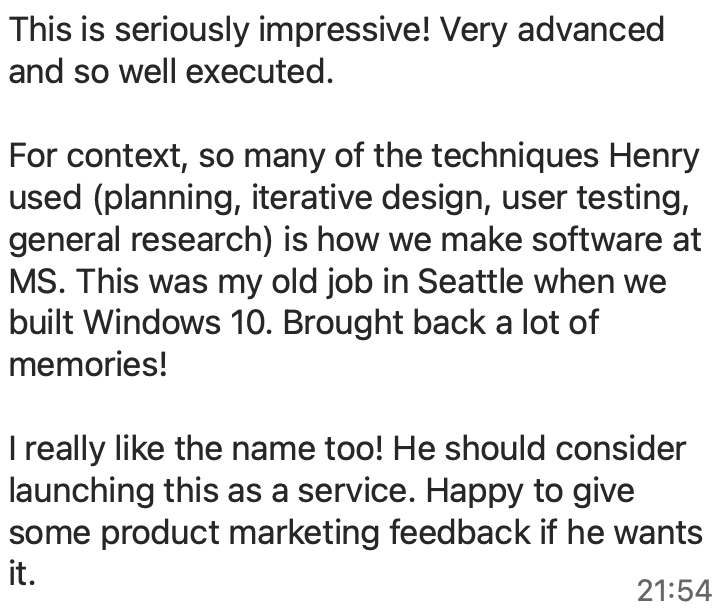
\includegraphics[width=0.6\textwidth]{VideoPresentation/PresentationEvaluation/media/microsoft.png}
    \caption{Message from industry expert}
\end{figure}

I am definitely going to take him up on his offer and hope to further develop my project from here

I also received these messages from a friend who is now very excited to use my product for here daily notes. She had previously given me a lot of useful feedback regarding certain features such as my chemistry and maths epxression editors and I am glad to see she is now excited to use the final product.

\begin{figure}[H]
    \centering
    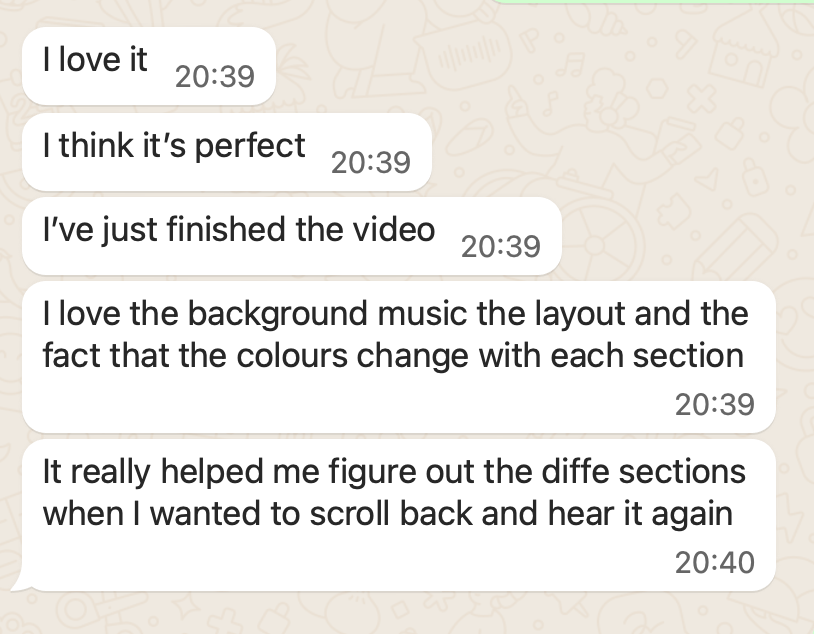
\includegraphics[width=0.6\textwidth]{VideoPresentation/PresentationEvaluation/media/friend.png}
    \caption{Message from friend}
\end{figure}


For more evaluation of my presentation and the production process please see my "Evaluation of markeplace presentation" section within my PPR above.